\begin{figure}[htb]
  \centering
  \caption{Spatial Distribution of Climate Damages}
  \label{fig:damage_maps}
  \begin{minipage}[t]{0.32\textwidth}
    \centering
    \small{A. Wage Damages ($\Delta w$)}
    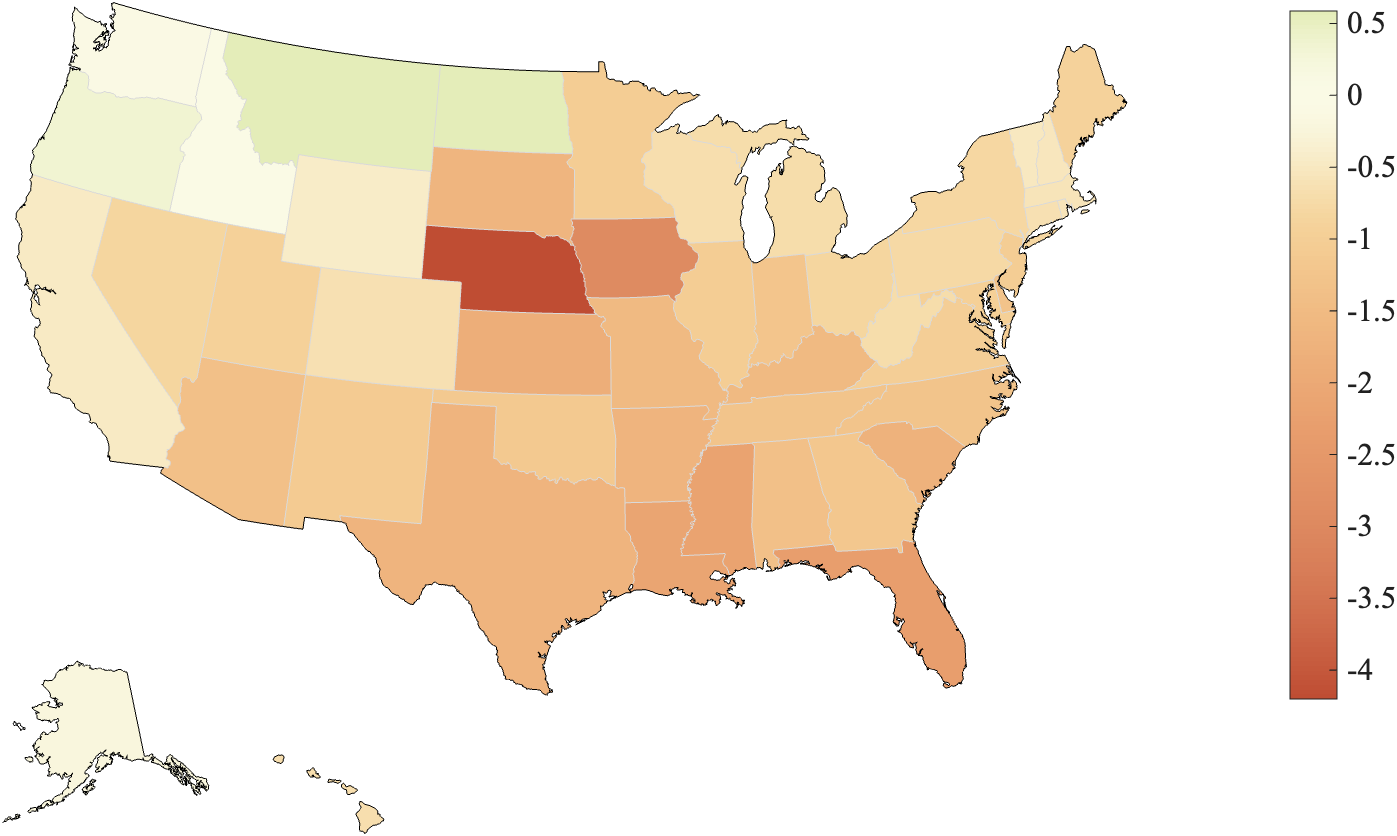
\includegraphics[width=\textwidth]{../Output/big_nu/graph_perfect_foresight/damage_maps/damage_maps_damage_wage.png}
  \end{minipage}\hfill
  \begin{minipage}[t]{0.32\textwidth}
    \centering
    \small{B. Amenity Damages ($\Delta A$)}
    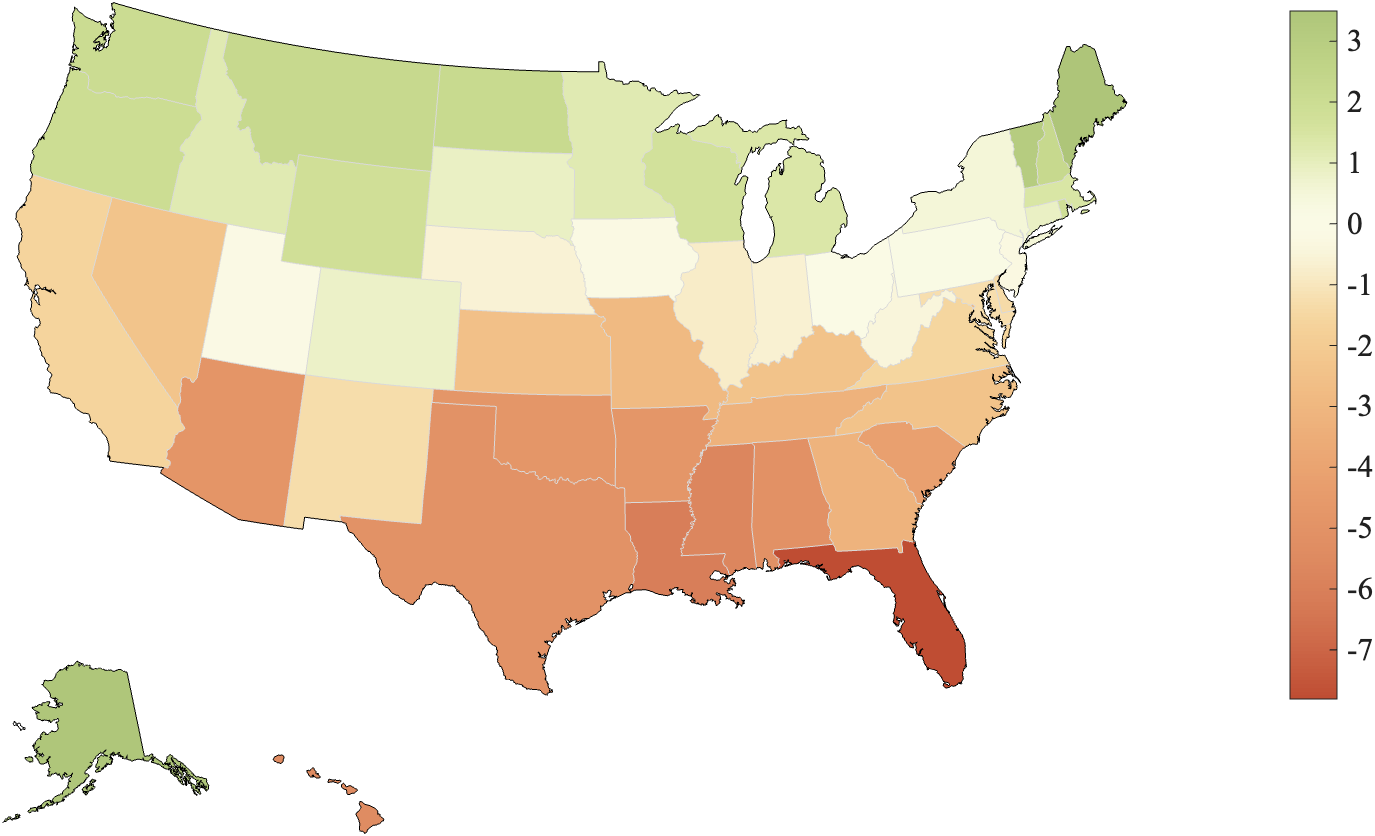
\includegraphics[width=\textwidth]{../Output/big_nu/graph_perfect_foresight/damage_maps/damage_maps_damage_amenity.png}
  \end{minipage}\hfill
  \begin{minipage}[t]{0.32\textwidth}
    \centering
    \small{C. Housing Damages ($\Delta q$)}
    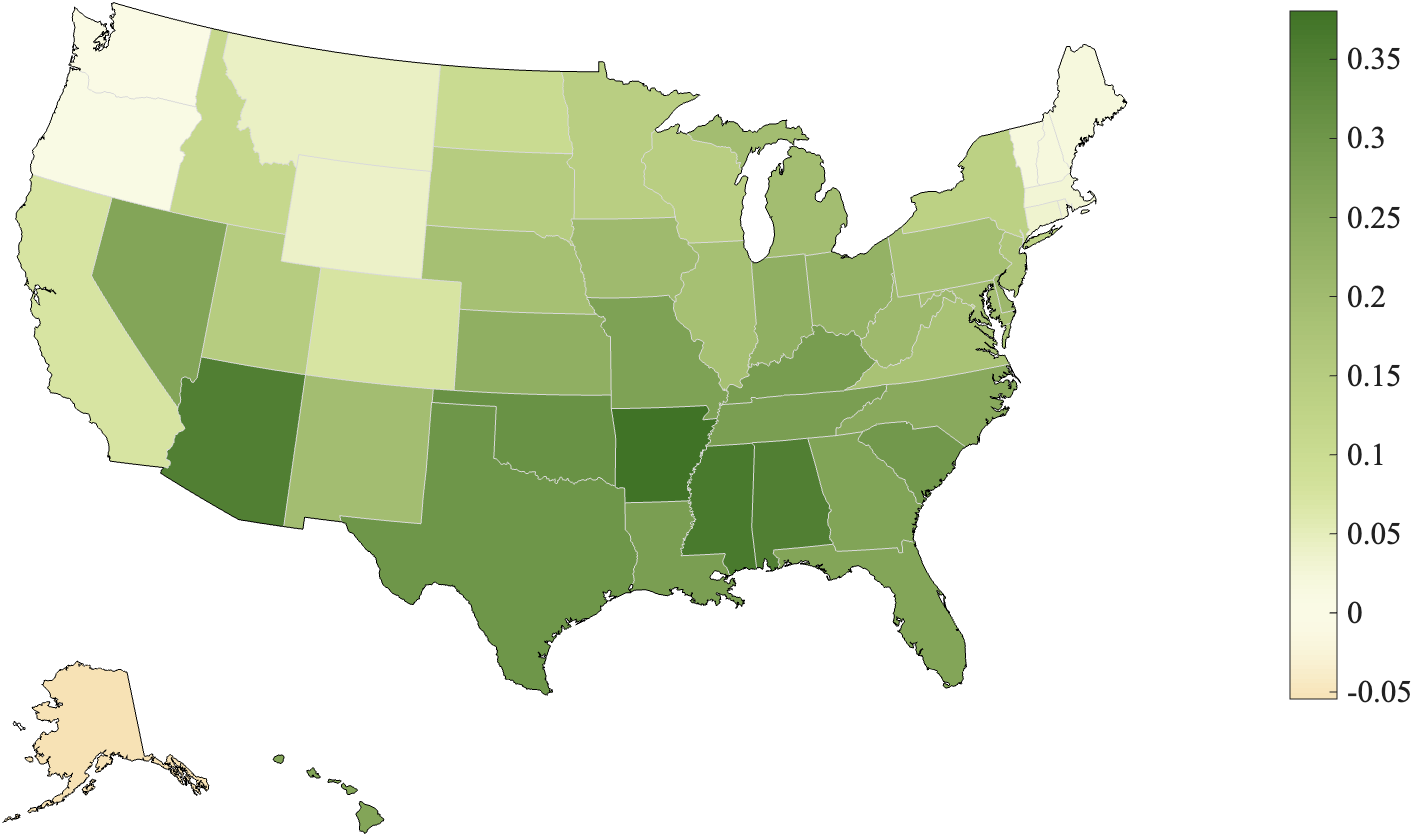
\includegraphics[width=\textwidth]{../Output/big_nu/graph_perfect_foresight/damage_maps/damage_maps_damage_housing.png}
  \end{minipage}
  \begin{minipage}{\textwidth}
  \vspace{0.5em}
  \footnotesize{\textbf{Note:} State-level spatial distribution of calibrated RCP 8.5 climate damage shocks across $J=51$ states. Panel~(a): percentage wage damage $\Delta w_\ell = \text{shock\_wage}_\ell \times 100$, where $w_{\ell, \text{term}} = w_{\ell, \text{init}}(1 + \text{shock\_wage}_\ell)$ combines labour productivity, agricultural yield, and coastal loss channels. Panel~(b): amenity loss expressed in consumption-equivalent percentage points, $\Delta A_\ell^{\text{CE}} = (\text{shock\_amenity}_\ell / \gamma) \times 100$, where $A_{\ell, \text{term}} = A_{\ell, \text{init}} - \text{shock\_amenity}_\ell$ based on temperature mortality and monetised crime rates. Panel~(c): percentage housing cost shock $\Delta q_\ell = \text{shock\_housing}_\ell \times 100$, where $q_{\ell, \text{term}} = q_{\ell, \text{init}}(1 + \text{shock\_housing}_\ell)$ through energy demand.} \end{minipage}
\end{figure}